


\usepackage{ragged2e}
\let\raggedright=\RaggedRight % for improved hypenation

\usepackage[italian]{babel}
\usepackage[utf8]{inputenc}

\setbeamertemplate{navigation symbols}{} 

\setbeamertemplate{footline}
{%
  \leavevmode%
  \hbox{\begin{beamercolorbox}[wd=.5\paperwidth,ht=2.5ex,dp=1.125ex,leftskip=.3cm plus1fill,rightskip=.3cm]{title in head/foot}%
    \usebeamerfont{author in head/foot}\insertshorttitle
  \end{beamercolorbox}%
  \begin{beamercolorbox}[wd=.5\paperwidth,ht=2.5ex,dp=1.125ex,leftskip=.3cm,rightskip=.3cm plus1fil]{author in head/foot}%
    \usebeamerfont{title in head/foot}\insertshortauthor\ -- \insertshortinstitute
  \end{beamercolorbox}}%
  \vskip0pt%
}

\usepackage{caption}
\usepackage{subcaption}

\title{LiquidFeedback: Democrazia Interattiva}
\author[Cal. \& Robotica]{Giuseppe Cal. \and Daniele Robotica}
\only<presentation>{\institute{Partito Pirata Italiano}}
\only<article>{\publishers{Partito Pirata Italiano}}
\date{30 settembre 2012}

\begin{document}

\begin{frame}
\maketitle

Se avete domande, \textsl{interrompeteci in \underline{qualsiasi} momento.}
\end{frame}

\section{Struttura del software}
\begin{frame}{Sezioni ed aree}
LiquidFeedback 2.x divide il campo decisionale in sezioni ed aree: 
\begin{columns}
\begin{column}{0.5\textwidth}
\begin{itemize}
\item Una \emph{sezione} (\emph{unit}) raggruppa insieme aree affini, come ad esempio, quelle relative all'amministrazione piuttosto che ai contenuti o alla produzione documentale.
\item Un'\emph{area} è un insieme più ristretto, utile a trattare in modo separato gli affari esteri e la regolamentazione dei trasporti, nell'esempio.
\end{itemize}
\end{column}
\begin{column}{0.5\textwidth}
\begin{figure}
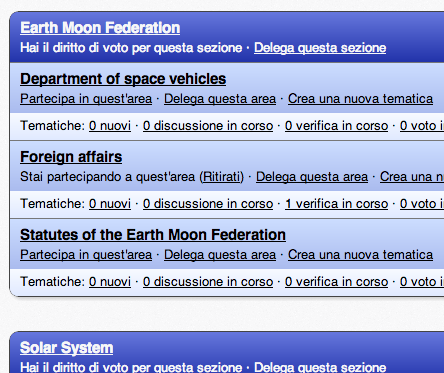
\includegraphics[width=0.95\textwidth]{pics/unitarea}
\caption{Le sezioni sulla federazione terra luna con le rispettive aree. Intravista, la sezione sul sistema solare.}
\end{figure}
\end{column}
\end{columns}
\end{frame}

\begin{frame}{Aree, ``partecipazione'' e quorum}
Per evitare che vengano discusse proposte poco interessanti, è richiesto che un certo numero di supporters portino avanti le proposte che ritengono interessanti.

Questo numero è regolabile in ogni area ed è proporzionale al numero di utenti che dicono (cliccando sull'apposito \emph{partecipa in quest'area}) di essere interessati ad un'area.
\begin{figure}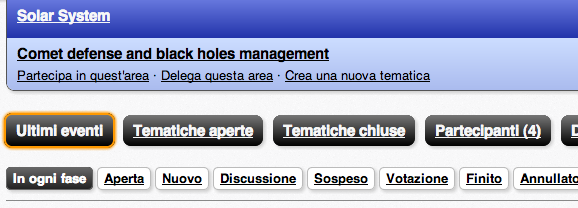
\includegraphics[width=0.8\textwidth]{pics/partecipa}
\caption{Come esprimere la propria ``partecipazione.''}
\end{figure}
\end{frame}

\begin{frame}[b]{Aree e deleghe}
\begin{columns}\begin{column}{.6\textwidth}
In alternativa alla partecipazione diretta, è possibile \textbf{impostare un fiduciario} che agirà in proprio nome all'interno di quell'area; o \textit{ignorarla del tutto, fidandosi di ciò che gli altri decidono}.\end{column}
\begin{column}{.4\textwidth}\begin{block}{Quorum}Anche delegando si concorre al calcolo della popolazione di un'area, e quindi dei quorum.\end{block}\end{column}
\end{columns}
\begin{figure}\centering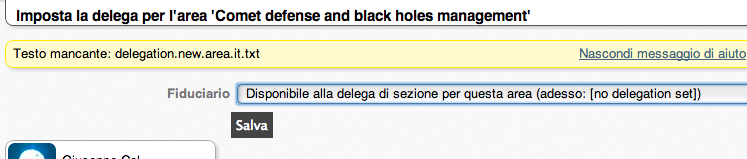
\includegraphics[width=0.99\textwidth]{pics/delega}
\caption{Deleghi qualcuno scegliendo fra i tuoi contatti e salvando; di default, un'area eredita le impostazioni dalla sezione che la contiene.}
\end{figure}
\end{frame}

\begin{frame}{Seguire le aree}
Una volta scelte le aree che vogliamo seguire, torniamo alla home page. Da qui, cliccando su ``ultimi eventi'' possiamo vedere cosa succede nelle nostre aree preferite, ed anche in tutte le altre, giocando opportunamente con i filtri.
\begin{figure}
\centering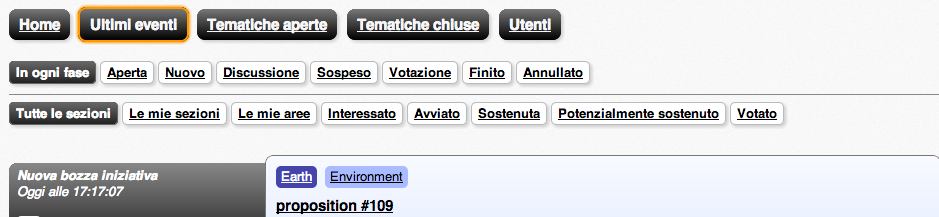
\includegraphics[width=0.99\textwidth]{pics/timeline-filters}
\caption{In alto, i filtri. In basso, gli eventi.}
\end{figure}
\end{frame}

\section{Processo decisionale}
\begin{frame}{Supportare una proposta esistente}
\begin{columns}
\begin{column}{.5\textwidth}
I pirati sono normalmente della gente molto figa, che non perde troppo tempo in chiacchiere; per il tuo ingresso ci sarà almeno una proposta in attesa di entrare in discussione o verifica.
\begin{itemize}
\item Sostenendo una proposta le consenti di andare al voto.
\item Sostenere una proposta significa anche esprimere interesse per il tema che la contiene, consentendogli di entrare in discussione.
\end{itemize}
\end{column}
\begin{column}{.5\textwidth}\begin{figure}\centering\includegraphics[width=\textwidth]{pics/init}
\caption{``Sostieni questa iniziativa.''}
\end{figure}\end{column}
\end{columns}
\end{frame}

\begin{frame}{Creare una nuova proposta... }
Hai avuto un'idea geniale per un punto che ancora manca nel programma del PP-IT, e vuoi che sia inclusa.
\begin{itemize}\item scegli l'area adatta;\item clicca su ``Crea una nuova tematica;''\item scrivi e salva.\end{itemize}
\begin{figure}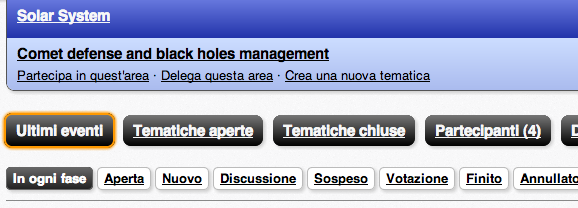
\includegraphics[width=0.8\textwidth]{pics/partecipa}
\caption{``Crea una nuova tematica''}
\end{figure}
\end{frame}

\begin{frame}{...o rispondere ad una già presente}
\begin{columns}
\begin{column}{.5\textwidth}Hai visto un'iniziativa. Ma non ti piace o vuoi comunque migliorarla. Bene, durante la fase di discussione hai due possibilità:\begin{itemize}\item Scrivere un'alternativa: link apposito, quindi scrivi e salva; \item Suggerire un'emendamento, tassativo o meno. \end{itemize}
\begin{block}{Eppure...}
Le due cose non sono mutuamente esclusive. Puoi suggerire e insieme proporre tutte le alternative che vuoi. 
\end{block}
\end{column}
\begin{column}{.5\textwidth}\begin{figure}\includegraphics[width=\textwidth]{pics/init}
\caption{``Crea un'iniziativa alternativa,'' ``Nuovo suggerimento''}
\end{figure}\end{column}
\end{columns}
\end{frame}

\begin{frame}{Discutere con i pirati}
Adesso hai presentato la tua iniziativa. C'è chi l'ha gradita e ti ha dato supporto, c'è chi ha suggerito emendamenti, c'è chi ha proposto un'antitetica alternativa. \begin{itemize}\item Le alternative ti fanno vedere in che modo i tuoi colleghi pirati affrontano lo stesso problema. \item I suggerimenti ti dicono che pensano della tua!\begin{itemize}\item {\bfseries Sono valutati}: di ogni suggerimento sai qual è il numero dei pirati favorevoli, nei due gradi, e quello dei contrari. \item è {\bfseries valutata anche la loro implementazione}.\end{itemize}\end{itemize} \begin{figure}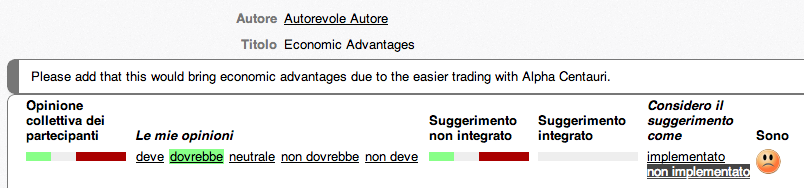
\includegraphics[width=\textwidth]{pics/suggerimento}
\caption{Un suggerimento nel dettaglio}
\end{figure}
\end{frame}

\begin{frame}{Votare}
Terminata la fase di discussione, la tematica entrerà in una fase di congelamento durante la quale sarà possibile soltanto leggere, dare/togliere supporto e presentare iniziative alternative di emergenza (che non potranno essere discusse).

Tutte le iniziative che raggiungono un determinato quorum di supporto vengono presentate sulla scheda per il voto.
\begin{block}{Non è un semplice voto si/no oppure ``voto per questa.''}
Sulla scheda va espressa una classifica di gradimento delle proposte, ``questa è la mia preferita,'' ``questa andrebbe comunque bene,'' ``questa è brutta, ma quelle sotto sono peggio,'' ``questa mi fa completamente schifo.''\end{block}
\end{frame}

\begin{frame}{La scheda}
\begin{figure}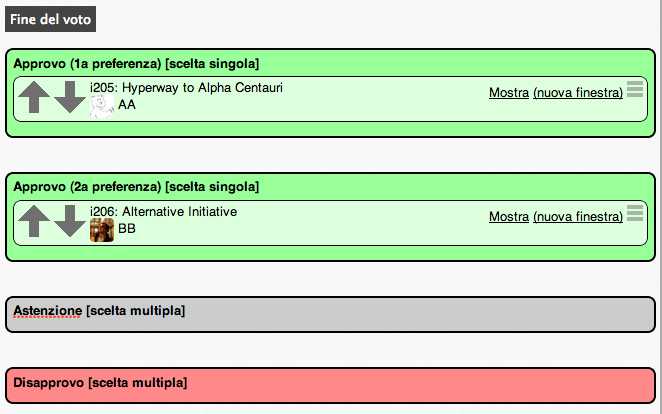
\includegraphics[width=.9\textwidth]{pics/scheda}
\caption{In basso, il pulsante per confermare il voto}
\end{figure}
\end{frame}

\begin{frame}{Metodo Schulze}
\begin{columns}
\begin{column}{.666\textwidth}
Prende in ingresso gli ordinamenti dalle schede e produce un ordinamento delle proposte candidate, in modo che se la maggior parte dei votanti ha preferito la proposta $A$ a quella $B$, la proposta $A$ sarà sopra la $B$ nell'ordinamento finale.

\alert{Quella proposta che è preferita ad ogni altra arriva in prima posizione  nell'ordinamento finale e quindi vince}.

\begin{block}{Nota bene}
Non valgono soltanto gli ``scontri diretti:'' viene considerata la connessione più debole sul percorso migliore.
\end{block}
\end{column}
\begin{column}{.333\textwidth}
\begin{figure}
\centering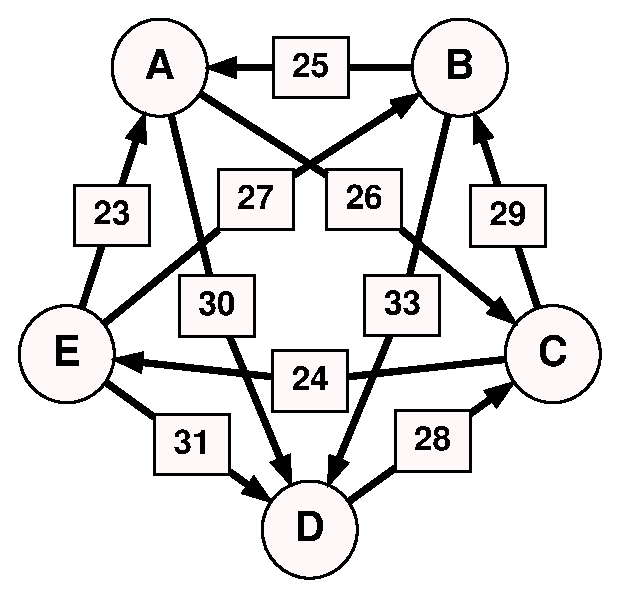
\includegraphics[width=\textwidth]{pics/Schulze_method_example1}
\caption{Grafo orientato con indicate le preferenze coppia a coppia fra le proposte. (Commons, CC-BY-SA)}
\end{figure}
\end{column}
\end{columns}
\end{frame}
\section{Dopo il voto}
\begin{frame}{Verificare i risultati}
Alla fine della fase di voto saranno disponibili ai votanti le schede di tutti, con l'indicazione di chi ha votato cosa.

\begin{itemize}\item Questi dati sono utilizzabili per verificare che la macchina non imbrogli i votanti, scegliendo al loro posto.\end{itemize}
\begin{figure}
	\begin{subfigure}[b]{.58\textwidth}
		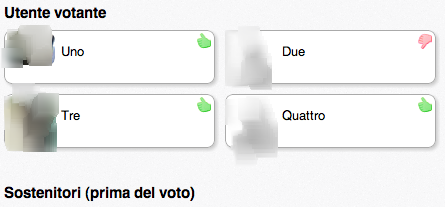
\includegraphics[width=\textwidth,]{pics/voters}
		\caption{Chi e come ha votato la proposta...}
	\end{subfigure}
	\begin{subfigure}[b]{.34\textwidth}
		\includegraphics[width=\textwidth]{pics/scheda-post}
		\caption{...in dettaglio}
	\end{subfigure}
\caption{La prima, sulla pagina della proposta. La seconda, cliccando sul pollice colorato dell'utente desiderato. Un pallino giallo indica astensione; uno sfondo arancione insegue il tuo voto.}
\end{figure}
\end{frame}

%\begin{frame}{Che fine ha fatto il mio voto?}
%\end{frame}

\begin{frame}{Voti palesi: problema?}
\begin{columns}
\begin{column}[t]{.5\textwidth}
\textbf{Contro}:\begin{itemize}
\item Posso pressarti a votare in un certo modo. Ma si vede.
\item Potresti non sapere cosa tu stesso hai votato, se deleghi qualcuno.
\item Potresti essere soggetto a ritorsioni.
\end{itemize}
\end{column}
\begin{column}[t]{.5\textwidth}
\textbf{Pro}:\begin{itemize}
\item Eventuali lobby diventano subito manifeste.
\item Puoi vedere cosa votano i tuoi delegati, anche prima di decidere che diventino tali.
\item \alert{Trasparenza della macchina di voto}.
\end{itemize}
\end{column}
\end{columns}\pause
\begin{block}{La risposta è NO}
LiquidFeedback è pensato per ricalcare le procedure di un'assemblea dove si vota per alzata di mano, come un parlamento elettronico. \emph{Non introduce problemi che non esistessero già}.
\end{block}
\end{frame}

\begin{frame}{Trasparenza della macchina di voto}
\begin{block}{LiquidFeedback è una scatola di vetro}
\begin{description}
\item[Trasparente:] puoi vedere ogni cosa che succede al suo interno. Non esistono dati segreti, puoi ricalcolare i suoi risultati armato di sole carta, matita e matematica.
\item[Deterministico:] sai esattamente cosa uscirà fuori, date le condizioni iniziali. LiquidFeedback non è un oracolo, serve ``soltanto'' a facilitare i processi decisionali.
\end{description}
\end{block}
\begin{itemize}
\item LQFB è pensato in modo che l'affidabilità della macchina sul quale viene installato non sia un fattore critico.
\item \alert{L'unico fattore decisivo sono i suoi utenti}.
\end{itemize}
\end{frame}

\begin{frame}{È bellissimo: voglio diventar pirata anch'io!}

\begin{center}
{\huge \texttt{info@partito-pirata.it \\~\\ http://votopirata.it}}
\end{center}

\end{frame}
\end{document}
